%% Week 42 -- Backpropagation and the output layers once more, then neural
%% networks for differential equations: ODEs, the diffusion equation, and
%% physics-informed neural networks.
%% Sources: Chapter 8 of the book for the reminder (Sections 8.4, 8.6, 8.8.4-
%% 8.8.5, 8.11, 8.13), Chapter 5 for the softmax and the cross entropy, and
%% Chapter 9 for everything after the first half hour: Sections 9.1-9.5
%% (trial solution, derivatives with respect to the input, the three ODEs),
%% 9.6-9.7 (PDEs and the diffusion equation), 9.9 (when is it worth doing)
%% and 9.10 (physics-informed networks, the inverse problem).
%% Part 1 (30 min) is the reminder of week 41 with a code demonstration on the
%% Runge function and on MNIST; Part 2 (25 min) the ordinary differential
%% equations; Part 3 (15 min) the diffusion equation; Part 4 (20 min) PINNs.
%% Equation, figure, section and table numbers are those of book.aux
%% (chapter 9 unchanged since 2026-09-06, chapter 8 as of 2026-09-23).
%% Figures week42_*.pdf are produced by make_week42_figures.py, which imports
%% the week-41 network from make_week41_figures.py; the same code appears
%% verbatim in week42.ipynb.  Book figures come from BookFigures/chapter08_*
%% and chapter09_*.
%% Tuesday (week42tuesday.tex/ipynb) has ONE case: the backward pass, the
%% structure of exercisesweek42.ipynb (deadline Friday October 16).
%% Build:  pdflatex week42slides.tex  (twice)
\documentclass[10pt,aspectratio=169]{beamer}
\usetheme{red_plain}
\usepackage[T1]{fontenc}
\usepackage[utf8]{inputenc}
\usepackage{amsmath,amssymb,bm}
\usepackage{graphicx}
\usepackage{listings}
\usepackage{xcolor}
\usepackage{booktabs}
\graphicspath{{../BookFigures/chapter08_neural_networks/}{../BookFigures/chapter09_differential_equations/}{./}}

%% ---- code listings
\definecolor{codebg}{rgb}{0.97,0.97,0.97}
\lstset{language=Python,basicstyle=\ttfamily\scriptsize,backgroundcolor=\color{codebg},
  keywordstyle=\color{blue!70!black}\bfseries,commentstyle=\color{green!45!black},
  stringstyle=\color{red!60!black},showstringspaces=false,frame=single,
  framerule=0pt,xleftmargin=4pt,xrightmargin=4pt,breaklines=true,columns=fullflexible}

%% ---- the "pause and think" question frames
\newcounter{insight}
\newenvironment{insight}[1][]{%
  \stepcounter{insight}%
  \begin{frame}{Pause and think \arabic{insight}: #1}%
  \setbeamercolor{block title}{bg=structure.fg,fg=white}%
  \setbeamercolor{block body}{bg=structure.fg!8}%
  \small
}{\end{frame}}
\newcommand{\question}[1]{\begin{block}{Question}#1\end{block}}
\newcommand{\answer}[1]{\pause\begin{block}{Answer}#1\end{block}}
\newcommand{\hint}[1]{\pause{\small\emph{Hint: }#1}}

\setbeamertemplate{footline}[frame number]
\setbeamertemplate{blocks}[rounded][shadow=false]
\setbeamercovered{invisible}

\title{Week 42: From Backpropagation to Differential Equations}
\subtitle{The network of week 41 once more -- activations, output layers, the
  algorithm -- and then the same network solving ordinary and partial
  differential equations, ending with physics-informed neural networks\\[3pt]
  \small With pauses for questions}
\author{Morten Hjorth-Jensen}
\institute{Department of Physics and Center for Computing in Science Education,\\
  University of Oslo, Norway}
\date{}

\begin{document}

\begin{frame}
\titlepage
\end{frame}

\begin{frame}{Plan for week 42}
\footnotesize
\textbf{Monday lecture (2$\times$45 min):}
\begin{itemize}
  \item \textbf{First 30 min, the reminder from last week:} the forward pass,
        the four equations of backpropagation and how to set the algorithm up;
        the activation functions and why there must be one; the output
        activation for regression (linear), binary classification (sigmoid)
        and $K$ classes (softmax), each paired with its cost -- with the code
        of week 41 run on the Runge function and on MNIST (Sections 8.6,
        8.8.4--8.8.5, 8.11, 8.13)
  \item \textbf{Differential equations without data (Chapter 9):} the trial
        solution and the residual as a cost, derivatives of the network with
        respect to its \emph{input}, and three ordinary differential equations
        -- exponential decay, logistic growth, the Poisson equation --
        checked against the exact solution, forward Euler and finite
        differences (Sections 9.1--9.5)
  \item \textbf{A partial differential equation:} the diffusion equation in
        one dimension with a trial solution that satisfies all conditions
        exactly (Sections 9.6--9.7)
  \item \textbf{Physics-informed neural networks:} the conditions as soft
        constraints, what that costs in accuracy, and what it buys -- an
        unknown diffusion coefficient recovered from forty noisy measurements
        (Section 9.10)
\end{itemize}
\textbf{Tuesday (flipped classroom):} your questions, then \emph{one} case:
the backward pass of this week's exercises -- shapes, the feed-forward
repetition, the four equations in code (\textbf{deadline Friday October
16}).\\[2pt]
\textbf{Reading:} Chapter 9, Sections 9.1--9.7 and 9.9--9.10; Sections 8.6,
8.8 and 8.11 as a reminder.  Goodfellow et al.\ Chapter 6; Raschka et al.\
Chapter 11; Lagaris, Likas and Fotiadis (1998); Raissi, Perdikaris and
Karniadakis (2019).
\end{frame}

%% ====================================================================
%% Part 1: the reminder (30 min)
%% ====================================================================

\begin{frame}{Where we were: the forward pass and the four equations (8.5, 8.8.4)}
\begin{columns}[T]
\begin{column}{0.27\textwidth}
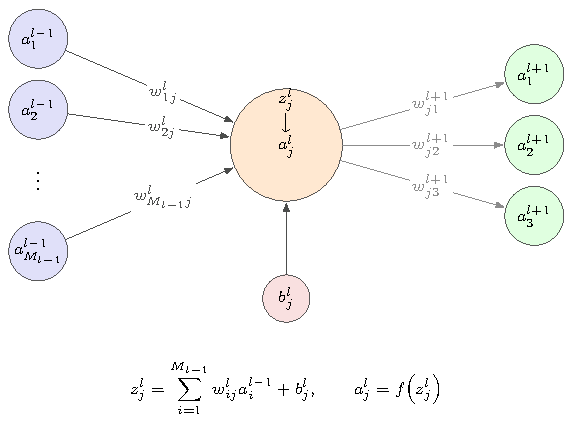
\includegraphics[width=0.95\textwidth]{8-node}\par
\vspace{2pt}
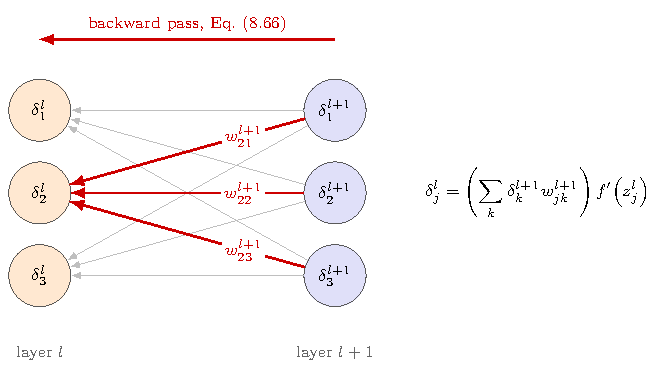
\includegraphics[width=0.95\textwidth]{8-backprop}\par
\scriptsize Book Figures 8.6 and 8.13: the same graph, arrows reversed.
\end{column}
\begin{column}{0.71\textwidth}
\scriptsize
\textbf{Forward}, Eq.~(8.21), samples in the rows of $\bm{A}^{0}=\bm{X}$,
$\bm{W}^{l}$ of shape $(M_{l-1},M_l)$, the \emph{output} activation in the
last layer, every $\bm{Z}^{l}$ and $\bm{A}^{l}$ stored:
$\bm{Z}^{l}=\bm{A}^{l-1}\bm{W}^{l}+\bm{b}^{l}$, $\bm{A}^{l}=f(\bm{Z}^{l})$,
$l=1,\dots,L$.
\begin{block}{Backward: the four equations (8.65)--(8.68), for a batch}
\scriptsize
\begin{align*}
  \bm{\Delta}^{L}&=f'(\bm{Z}^{L})\circ\partial C/\partial\bm{A}^{L}
   &&\text{start; }\bm{A}^{L}-\bm{Y}\text{ for the natural pairings (8.69)}\\[1pt]
  \bm{\Delta}^{l}&=\bigl(\bm{\Delta}^{l+1}(\bm{W}^{l+1})^{T}\bigr)\circ f'(\bm{Z}^{l})
   &&\text{carry back through }\bm{W}^{T}\text{, modulate by }f'\\[1pt]
  \partial C/\partial\bm{b}^{l}&=\textstyle\sum_{\text{samples}}\bm{\Delta}^{l}
   &&\text{bias: the error itself}\\[1pt]
  \partial C/\partial\bm{W}^{l}&=(\bm{A}^{l-1})^{T}\bm{\Delta}^{l}
   &&\text{weight: error }\times\text{ the entering signal}
\end{align*}
\end{block}
\textbf{The rule.}  $\delta_j^{l}=\partial C/\partial z_j^{l}$ is the error
of a node; the gradient of a weight is the error at the node it arrives at
times the signal at the node it leaves.  Two transposes in two different
places: $(\bm{W}^{l+1})^{T}$ sums over the \emph{next layer},
$(\bm{A}^{l-1})^{T}$ over the \emph{samples}.  The whole gradient costs
about two forward passes, whatever the number of parameters (Proposition
4.2) -- and a hand-written backward pass is always checked against finite
differences or \texttt{jax.grad}.
\end{column}
\end{columns}
\end{frame}

\begin{frame}[fragile]{Setting the algorithm up, and the code it became (8.8.5, 8.13)}
\vspace{-3pt}
\begin{columns}[T]
\begin{column}{0.44\textwidth}
\begin{block}{Five decisions before the first iteration}
\scriptsize
\begin{enumerate}
  \item The architecture: \texttt{sizes = [784, 100, 10]}.
  \item The hidden activation $f$ -- and its derivative $f'$, which is what
        (8.66) uses.
  \item The output activation, dictated by the \emph{range} of the target,
        and the cost, dictated by its \emph{distribution} (Section 3.6);
        penalties and their $\lambda$.
  \item The optimiser (week 38) and its learning rate $\gamma$, the minibatch
        size $M$, the number of epochs.
  \item The initialisation: variance $1/M_{l-1}$ or $2/M_{l-1}$ (8.73--8.74),
        never all zeros, never $\mathcal{N}(0,1)$ with $784$ inputs.
\end{enumerate}
\end{block}
\begin{block}{Each iteration, on a minibatch}
\scriptsize
forward pass storing $\bm{Z}^{l},\bm{A}^{l}$ $\to$ output error $\to$
backward pass $\to$ gradients $\to$ update $w\leftarrow w-\gamma\,\partial
C/\partial w$ (8.70).  Then \emph{check the gradient}: finite differences
(4.102) or \texttt{jax.grad}.
\end{block}
\end{column}
\begin{column}{0.56\textwidth}
\lstset{basicstyle=\ttfamily\tiny}
\begin{lstlisting}
def feed_forward(X, layers, hidden_activation="sigmoid", head="mse"):
    f, _ = ACTIVATIONS[hidden_activation]
    a, z = [X], []
    for l, (W, b) in enumerate(layers):
        zl = a[-1] @ W + b                       # Eq. (8.21)
        z.append(zl)
        a.append(OUTPUT[head](zl) if l == len(layers) - 1 else f(zl))
    return z, a

def backpropagation(X, Y, layers, hidden_activation="sigmoid", head="mse", lmbd2=0.0, lmbd1=0.0):
    _, fp = ACTIVATIONS[hidden_activation]
    n = X.shape[0]
    z, a = feed_forward(X, layers, hidden_activation, head)
    delta = (a[-1] - Y)/n                         # Eq. (8.69), all three heads
    grads = [None]*len(layers)
    for l in range(len(layers) - 1, -1, -1):
        W, _ = layers[l]
        dW = a[l].T @ delta + 2.0*lmbd2*W + lmbd1*np.sign(W)   # (8.68) + penalties
        db = np.sum(delta, axis=0)                 # (8.67)
        grads[l] = (dW, db)
        if l > 0:
            delta = (delta @ W.T) * fp(z[l - 1])  # (8.66)
    return grads
\end{lstlisting}
\scriptsize
\texttt{ACTIVATIONS} holds $(f,f')$ pairs, \texttt{OUTPUT} the three heads
\texttt{identity}, \texttt{sigmoid}, \texttt{softmax}; \texttt{train} loops
over epochs and minibatches.  Today we add \emph{one} row to
\texttt{ACTIVATIONS}: \texttt{"tanh": (tanh, tanh\_prime)}.  Part 2 says why.
\end{column}
\end{columns}
\end{frame}

\begin{frame}{Activation functions: what matters is the derivative (Section 8.6, Figure 8.9)}
\begin{columns}[T]
\begin{column}{0.5\textwidth}
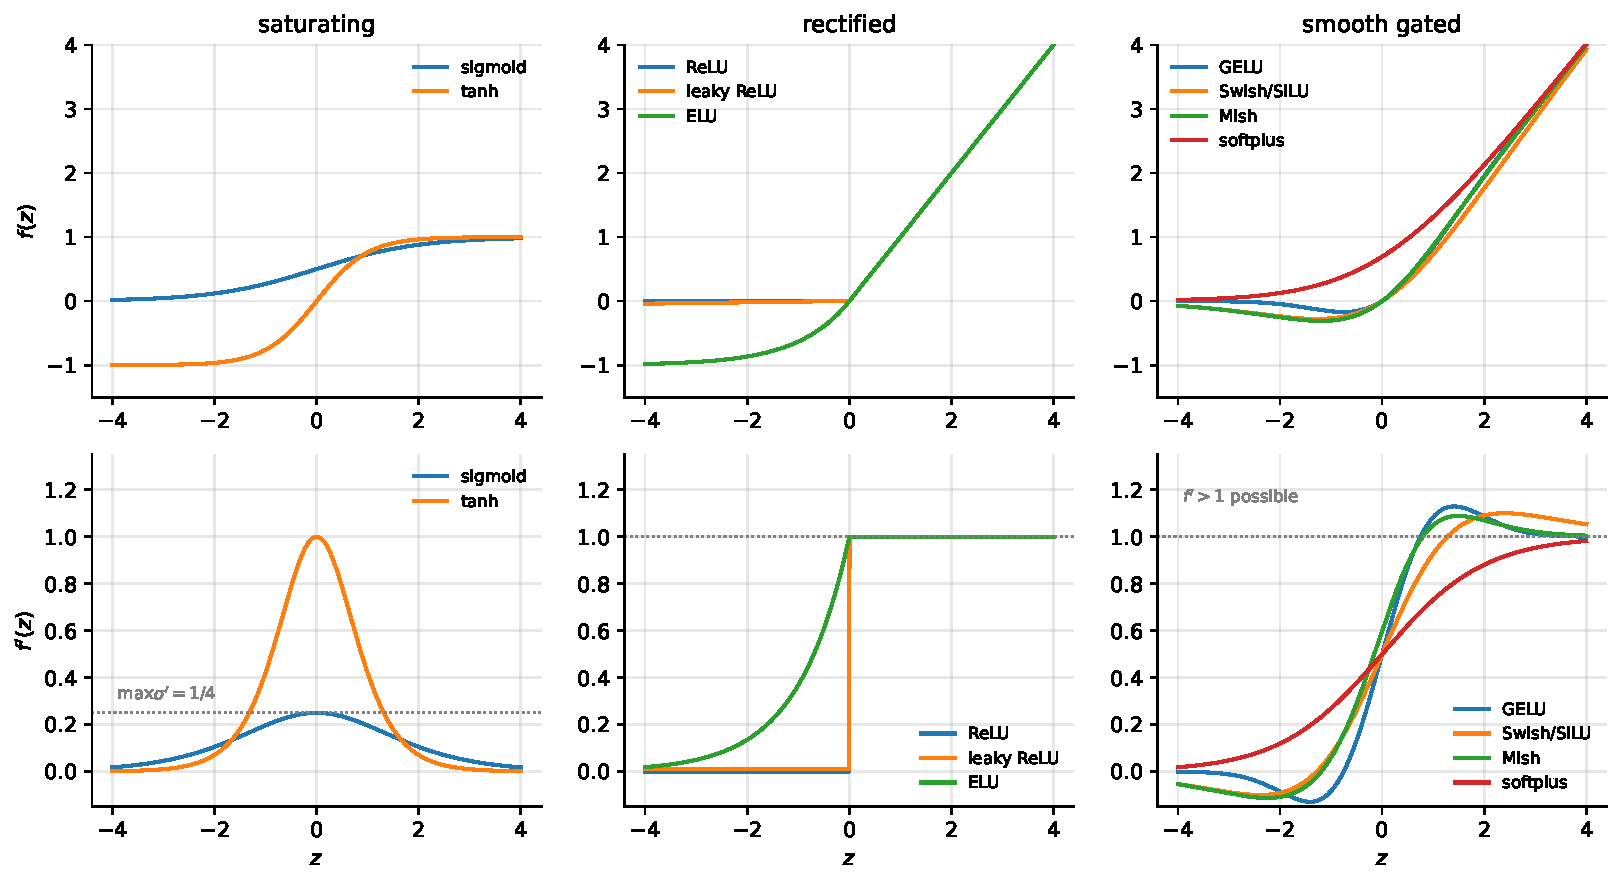
\includegraphics[width=\textwidth]{activation_families}\par
\scriptsize Nine activations in three families (top) and their derivatives
(bottom); dotted lines at $\max\sigma'=\frac14$ and at $f'=1$.
\end{column}
\begin{column}{0.5\textwidth}
\scriptsize
\textbf{Saturating} (8.22): $\sigma(z)=1/(1+e^{-z})$,
$\sigma'=\sigma(1-\sigma)\le\frac14$; $\tanh(z)=2\sigma(2z)-1$,
$\tanh'=1-\tanh^{2}\le1$, centred on zero -- always the better of the two in
a hidden layer.  Both have $f'\approx0$ for $|z|$ large: a saturated unit
stops learning, and $L$ sigmoid layers multiply the error by at most $4^{-L}$
(8.71).\\[3pt]
\textbf{Rectified} (8.23)--(8.25): $\mathrm{ReLU}(z)=\max(0,z)$, $f'=1$ on
the active side -- the gradient passes undiminished, half the units are
exactly zero; \emph{dying ReLU} when the input is negative for every sample.
Leaky ReLU, ELU repair the dead side.  \textbf{Smooth gated}
(8.26)--(8.28): GELU $z\Phi(z)$, Swish $z\sigma(z)$ -- ReLU without the kink.
\begin{block}{Two rules, and a third for today}
\scriptsize
(i) The hidden activation must be non-linear -- Section 8.4: \emph{not a
polynomial} -- or the network is one linear map.  (ii) In the backward pass
only $f'$ appears, so pick one whose derivative does not vanish where the
units live.  (iii) When the \emph{output} must be differentiated with respect
to the \emph{input}, $f''$ appears too -- and for the whole rectified family
$f''\equiv0$.  Hence $\tanh$ in Part 2.
\end{block}
\end{column}
\end{columns}
\end{frame}

\begin{frame}{Why a hidden layer with a non-linear activation fits a non-linear function (Section 8.4)}
\small
\begin{columns}[T]
\begin{column}{0.5\textwidth}
\begin{block}{The theorem, in its sharp form}
\footnotesize
A network with one hidden layer and a linear output is a universal
approximator -- any continuous $F$ on a compact set to any accuracy
$\epsilon$ (8.3) -- \emph{if and only if} the hidden activation is not a
polynomial (Leshno et al.\ 1993).  Cybenko proved it for sigmoids, Hornik for
anything bounded and non-constant, and in mean square (8.5) rather than
uniformly, which is the statement a statistician wants.
\end{block}
\begin{block}{What it does not say}
\footnotesize
Nothing about \emph{how many} units, nothing about whether gradient descent
\emph{finds} the weights: representability is not learnability (Section
8.4.4).  Polynomials, Fourier series and splines are universal too; what
distinguishes networks is depth -- Section 8.4.3 shows a function a deep
network represents with a polynomial number of units that a shallow one
needs exponentially many for.
\end{block}
\end{column}
\begin{column}{0.48\textwidth}
\begin{block}{A constructive version for ReLU in one dimension (8.6)--(8.8)}
\footnotesize
$g(x)=c+\sum_{i=1}^{N}v_i\,\mathrm{ReLU}(w_ix+b_i)$ is continuous and
piecewise linear with at most $N+1$ pieces, the kinks at $-b_i/w_i$ (Lemma
8.1) -- and conversely every such function is a one-hidden-layer ReLU
network.  Put the kinks at $N+1$ equally spaced knots and choose the
$v_i$ as the \emph{changes of slope} of the chords, Eq.~(8.8): the network
is the piecewise-linear interpolant, and for an $L$-Lipschitz $F$ on $[a,b]$
\[
  \sup_x|F(x)-g(x)|\le\frac{L(b-a)}{2N}\qquad\text{(8.7)}.
\]
A hidden unit is a kink, the output layer adds kinks with weights, and the
non-linearity is what lets a sum of them bend; with sigmoids each unit is a
smooth step.
\end{block}
\end{column}
\end{columns}
\end{frame}

\begin{frame}{Example A: the Runge function with ReLU, sigmoid and tanh hidden units (\texttt{week42\_runge.pdf})}
\centering
\includegraphics[width=0.98\textwidth]{week42_runge}\par
\vspace{-4pt}
\raggedright\scriptsize
The data of Project 1 ($n=100$, $\sigma=0.1$, seed 2026, a separate test set),
the $1$--$50$--$1$ network of week 41 with the linear output and the
half-squared error, plain gradient descent, $20\,000$ steps.  \textbf{(a)}
Test MSE $0.0094$ (ReLU, $\gamma=0.1$), $0.0124$ (sigmoid, $\gamma=0.2$),
$0.0111$ (tanh, $\gamma=0.1$); the noise variance is $0.01$, so all three
have found the function.  \textbf{(b)} ReLU is at the noise floor after a
few hundred steps; the sigmoid network first climbs to $C=30$ and needs
$10^{4}$ steps; tanh is in between -- the derivative up to $1$ instead of
$\frac14$ and the centred output.  \textbf{(c)} The ten largest of the fifty
ReLU units, each a kink $w_j^{2}\,\mathrm{ReLU}(w_j^{1}x+b_j^{1})$; all fifty
kinks lie inside $[-1,1]$, and their sum plus $b^{2}$ (blue) \emph{is} the
network: a piecewise-linear function that bends where the Runge function
does -- Lemma 8.1 after training rather than by construction.
\end{frame}

\begin{insight}[how many ReLU units does the Runge function need?]
\question{Theorem 8.2 guarantees $\sup|F-g|\le L(b-a)/(2N)$ for the
interpolating network with $N$ units.  For $F(x)=1/(1+25x^{2})$ on $[-1,1]$
the steepest slope is $L=\max|F'|\approx3.25$ (at $x=\pm0.115$).  How many
units does the bound require for an error of $0.01$, and how many did
gradient descent use to reach the noise floor?  Why the difference -- and
what would the \emph{same} network with the identity as hidden activation
have fitted?}
\answer{$N\ge L(b-a)/(2\cdot0.01)=3.25\cdot2/0.02=325$ units for the
guarantee; the trained network used $50$ (and week 41's $\ell_1$ run kept
only $10$ of them).  The bound is a worst case for \emph{equally spaced}
kinks and \emph{any} $L$-Lipschitz function; training puts the kinks where
the function bends and leaves the flat tails to one or two units each, so
the pieces are used far more economically -- Figure (c).  That is the gap
between a representability bound and what an optimiser finds, in the
favourable direction for once.  With the identity as hidden activation the
network is $g(x)=\bm{w}^{2T}(\bm{w}^{1}x+\bm{b}^{1})+b^{2}=\alpha x+\beta$:
a straight line, fifty-one parameters for a two-parameter model, and the
best fit to the Runge data is the horizontal line at the mean, MSE
$0.10$.  No kinks without a non-linearity; Section 8.4 made it an
if-and-only-if.}
\end{insight}

\begin{frame}{Output activations: three tasks, three heads, one output error (Sections 8.11, 5.3, 5.6)}
\footnotesize
The output activation is dictated by the \emph{range} of the target, the
cost by its \emph{distribution}; for the natural pairings the backward pass
starts with prediction minus target, Eq.~(8.69).
\begin{center}
\scriptsize
\setlength{\tabcolsep}{4pt}
\setlength{\tabcolsep}{3pt}
\begin{tabular}{@{}lllll@{}}
\toprule
Task & Output activation & Loss $L$ (one sample) & Likelihood of & $\bm{\delta}^{L}$\\
\midrule
regression, $y\in\mathbb{R}$ & linear, $a^{L}=z^{L}$ & $\tfrac12(a^{L}-y)^{2}$, (8.32) & a Gaussian (3.6) & $a^{L}-y$\\[2pt]
binary, $y\in\{0,1\}$ & sigmoid, $a^{L}=\sigma(z^{L})$ & $-y\ln a^{L}-(1-y)\ln(1-a^{L})$, (5.13) & a Bernoulli & $a^{L}-y$\\[2pt]
$K$ classes, $\bm{y}$ one-hot & softmax (8.75), $a_k^{L}=e^{z_k^{L}}/\sum_le^{z_l^{L}}$ & $-\sum_ky_k\ln a_k^{L}=-\ln a_{k^{*}}^{L}$, (5.28) & a categorical & $\bm{a}^{L}-\bm{y}$\\
\bottomrule
\end{tabular}
\end{center}
\begin{columns}[T]
\begin{column}{0.5\textwidth}
\begin{block}{The two cancellations}
\scriptsize
Sigmoid: $\partial L/\partial a=(a-y)/[a(1-a)]$ and $\sigma'=a(1-a)$ --
the $\sigma'$ that shrinks every squared-error gradient is divided out.
Softmax: the Jacobian $\partial a_k/\partial z_j=a_k(\delta_{kj}-a_j)$ is not
diagonal, but
$\delta_j^{L}=\sum_k(-y_k/a_k)\,a_k(\delta_{kj}-a_j)=-y_j+a_j\sum_ky_k=a_j-y_j$.
The $a_k$ cancels the $1/a_k$ of the logarithm, $\sum_ky_k=1$ does the rest.
Linear + squared error: $f'=1$, nothing to cancel.
\end{block}
\end{column}
\begin{column}{0.48\textwidth}
\begin{block}{What the heads \emph{mean}}
\scriptsize
A linear output can be $7$; a sigmoid output is a probability
$p(y=1\mid\bm{x})$; a softmax output is a \emph{distribution} over $K$
classes, positive and summing to one, computed from scores $z_k$ that are
only defined up to a common shift (subtract $\max_kz_k$ before
exponentiating, Eq.~5.30).  Two classes: one sigmoid node or two softmax
nodes, the same model.  Logistic regression is the network with $L=1$;
a classification network is logistic regression on learned features.
\end{block}
\end{column}
\end{columns}
\end{frame}

\begin{frame}{Why the pairing matters: a sigmoid output with the squared error (\texttt{week41\_delta\_heads.pdf})}
\centering
\includegraphics[width=0.8\textwidth]{week41_delta_heads}\par
\vspace{-3pt}
\raggedright\footnotesize
One sigmoid output node, target $y=1$.  \textbf{(a)} The cross entropy
$-\ln\sigma(z)$ grows linearly for $z\to-\infty$, the squared error
saturates at $\frac12$.  \textbf{(b)} The output error that starts the
backward pass: $|a-y|\to1$ for the cross entropy, the more wrong the
stronger the signal; $|a-y|\,\sigma'(z)$ for the squared error, which
\emph{vanishes} where the network is confidently wrong -- at $z=-5$ a factor
$150$ smaller.  A saturated, wrong output node learns almost nothing from its
mistake.  For a real-valued target the linear output with the squared error
(grey) has no saturation at all.  The same mechanism, $f'$ multiplying the
error, is the vanishing-gradient problem of Section 8.9 one layer deep.
\end{frame}

\begin{frame}{Example B: the sigmoid and the softmax head on MNIST (\texttt{week42\_mnist.pdf})}
\centering
\includegraphics[width=0.98\textwidth]{week42_mnist}\par
\vspace{-4pt}
\raggedright\scriptsize
The code of week 41, unchanged.  \textbf{(a)} Binary: the $11\,982$ threes
and eights of the training set, a $784$--$32$--$1$ ReLU network with the
sigmoid output and the cross entropy, $\gamma=0.1$, minibatches of $100$,
ten epochs, one second: test accuracy $98.24\%$ on $1984$ images ($35$
wrong).  The output is a probability: $61$ test images have
$0.2<p<0.8$ -- the network \emph{says} it is unsure -- and the threshold
$0.5$ is a decision we add afterwards.  \textbf{(b)} Ten classes: the
$784$--$100$--$10$ network with the softmax and the multiclass cross
entropy, twenty epochs, $97.63\%$ as last week.  \textbf{(c)} What the
output layer actually produces: ten scores $z_k$ (grey, scaled) and the
softmax probabilities $a_k$ (red).  Top: a zero predicted with probability
$1.0000$ -- one score far above the rest, the softmax turns a gap into a
certainty.  Bottom: the least confident of the $10\,000$ test images, a one
predicted correctly with $24\%$, with $20\%$ and $19\%$ for the next two
classes -- three scores within a few tenths of each other.  The softmax is
shift-invariant: only the \emph{differences} of the scores matter.
\end{frame}

\begin{insight}[which of the two images trains the network?]
\question{The backward pass starts with $\bm{\delta}^{L}=\bm{a}^{L}-\bm{y}$,
Eq.~(8.69).  Write it out for the two test images of Figure (c): the zero
with $a_0=1.0000$, and the one with $a_1=0.24$, $a_k\approx0.20$ and $0.19$
for two other classes.  Which image moves the weights, by how much, and in
which direction?  Why does the softmax need the cross entropy for this to
work -- what would the squared error $\frac12\sum_k(a_k-y_k)^{2}$ have given
for the confident \emph{wrong} answers of last week's error gallery, the
``$97\%$ zero'' that was not a zero?}
\answer{For the zero, $\delta_0=1.0000-1\approx0$ and every other
$\delta_k=a_k\approx0$: the sample contributes essentially nothing to
$(\bm{A}^{L-1})^{T}\bm{\Delta}^{L}$ -- a confident correct answer is
\emph{finished} and the gradient ignores it.  For the one,
$\delta_1=0.24-1=-0.76$ and $\delta_k=+0.20,+0.19,\dots$ for the rivals: a
strong push that raises the score of class $1$ and lowers the others, and
the $K$ errors sum to zero (the shift that the softmax cannot see).  The
cross entropy makes the signal proportional to the \emph{probability
mass} on the wrong classes, however the scores are placed.  With the squared
error on the softmax, (8.65) keeps the Jacobian $a_k(\delta_{kj}-a_j)$ in the
output error, and for a confident wrong answer -- $a_{\text{wrong}}=0.97$,
$a_{\text{true}}=0.03$ -- every factor $a_k(1-a_k)$ is small: the network
would learn least from exactly the mistakes it is surest about.  The
pairing of (8.69) is not a convenience; it is what makes the confident
mistakes the \emph{loudest} ones.}
\end{insight}

%% ====================================================================
%% Part 2: ordinary differential equations (Sections 9.1-9.5)
%% ====================================================================

\begin{frame}{A network with no data: the equation is the cost (Section 9.1)}
\small
\begin{columns}[T]
\begin{column}{0.5\textwidth}
\begin{block}{The problem}
\footnotesize
An ordinary differential equation of order $n$, Eq.~(9.1),
$f\bigl(x,g(x),g'(x),\dots,g^{(n)}(x)\bigr)=0$, with initial or boundary
conditions that make the solution unique.  No labels: nobody hands us
$g(x_i)$.  What we have is the equation.
\end{block}
\begin{block}{The trial solution, Eq.~(9.2)}
\footnotesize
\[
  \boxed{\;g_t(x,P)=h_1(x)+h_2\bigl(x,N(x,P)\bigr)\;}
\]
$N(x,P)$ is our network with parameters $P$; $h_1$ alone satisfies the
conditions; $h_2$ is built so that the network's contribution
\emph{vanishes} wherever a condition is imposed.  Then the conditions hold
\emph{exactly, for every $P$} -- at initialisation, after a bad step, always.
The optimiser has one job: make the equation hold.
\end{block}
\end{column}
\begin{column}{0.48\textwidth}
\begin{block}{The cost, Eq.~(9.3): the mean squared residual}
\scriptsize
At $N$ \emph{collocation points} $x_i$ that we choose,
\[
  C(\bm{x},P)=\frac1N\sum_{i=1}^{N}
  \Bigl(f\bigl(x_i,g_t(x_i),g_t'(x_i),\dots\bigr)\Bigr)^{2}.
\]
Three remarks.  The $x_i$ are not measurements: place them anywhere, change
them at will.  It is a mean squared error, so Chapter 4 applies unchanged --
Adam of week 38, the residual in the role of the target.  It is \emph{not}
convex, and we shall see a run converge confidently to the wrong answer.
\end{block}
\begin{block}{What is new, and what is not}
\scriptsize
New: the residual needs $g_t'$, hence $\partial N/\partial x$ -- a derivative
with respect to the \emph{input}, not the parameters.  Not new: the network,
its initialisation, the optimiser, the parameter gradient.  The idea is
Lagaris, Likas and Fotiadis (1998); as \emph{physics-informed neural
networks} it is a large research area today.
\end{block}
\end{column}
\end{columns}
\end{frame}

\begin{frame}[fragile]{Differentiating the network with respect to its \emph{input}: forward mode (9.2, Eqs.~9.4--9.6)}
\vspace{-3pt}
\begin{columns}[T]
\begin{column}{0.46\textwidth}
\scriptsize
Differentiate the forward pass $\bm{z}^{l}=\bm{a}^{l-1}\bm{W}^{l}+\bm{b}^{l}$,
$\bm{a}^{l}=f(\bm{z}^{l})$ with respect to an input coordinate $x_k$, starting
from $\partial\bm{a}^{0}/\partial x_k=\bm{e}_k$:
\[
  \frac{\partial\bm{z}^{l}}{\partial x_k}=\frac{\partial\bm{a}^{l-1}}{\partial x_k}\bm{W}^{l},\qquad
  \frac{\partial\bm{a}^{l}}{\partial x_k}=f'(\bm{z}^{l})\circ\frac{\partial\bm{z}^{l}}{\partial x_k}\quad(9.5)
\]
and once more, with the product rule,
\[
  \boxed{\;\frac{\partial^{2}\bm{a}^{l}}{\partial x_k^{2}}
  =f''(\bm{z}^{l})\circ\Bigl(\frac{\partial\bm{z}^{l}}{\partial x_k}\Bigr)^{2}
  +f'(\bm{z}^{l})\circ\frac{\partial^{2}\bm{z}^{l}}{\partial x_k^{2}}\;}\quad(9.6)
\]
The derivatives travel \emph{forward} with the activations: one extra matrix
product per layer per order, three forward passes for $N,N',N''$.  This is
forward-mode AD (Section 4.14), and the right mode here: \emph{one} input,
many parameters -- the reverse of training, where there is one cost and many
parameters, which is why the parameter gradient still goes backwards.
\end{column}
\begin{column}{0.54\textwidth}
\lstset{basicstyle=\ttfamily\tiny}
\begin{lstlisting}
def network_derivs(layers, X, activation="tanh", k=0):
    """N, dN/dx_k, d2N/dx_k^2 by the forward recursions (9.5), (9.6)."""
    f, fp = ACTIVATIONS[activation]            # the week-41 table
    fpp = {"tanh": lambda z: -2.0*np.tanh(z)*(1.0 - np.tanh(z)**2),
           "sigmoid": lambda z: sigmoid_prime(z)*(1.0 - 2.0*sigmoid(z)),
           "relu": lambda z: np.zeros_like(z)}[activation]
    a = np.asarray(X, dtype=float)
    da = np.zeros_like(a) + (np.arange(a.shape[1]) == k)   # da0/dxk = e_k
    d2a = np.zeros_like(a)
    for l, (W, b) in enumerate(layers):
        z, dz, d2z = a @ W + b, da @ W, d2a @ W
        if l < len(layers) - 1:
            a, da, d2a = f(z), fp(z)*dz, fpp(z)*dz**2 + fp(z)*d2z
        else:                                   # linear output
            a, da, d2a = z, dz, d2z
    return a[:, 0], da[:, 0], d2a[:, 0]
\end{lstlisting}
\scriptsize
Three lines per layer added to \texttt{feed\_forward}, the activation table
of week 41 reused.  \textbf{Checked} against \texttt{jax.grad} of the same
network: $2\times10^{-16}$ in $N'$ and $N''$ for tanh, $10^{-17}$ for the
sigmoid, $0$ for ReLU -- that last zero is the next frame.  The hand
recursion is for understanding; for the PDEs we differentiate the
\emph{trial solution} itself by nested AD (next code frame).
\end{column}
\end{columns}
\end{frame}

\begin{frame}{The activation now matters more: $f''$ (Section 9.2, Figure 9.1)}
\begin{columns}[T]
\begin{column}{0.46\textwidth}
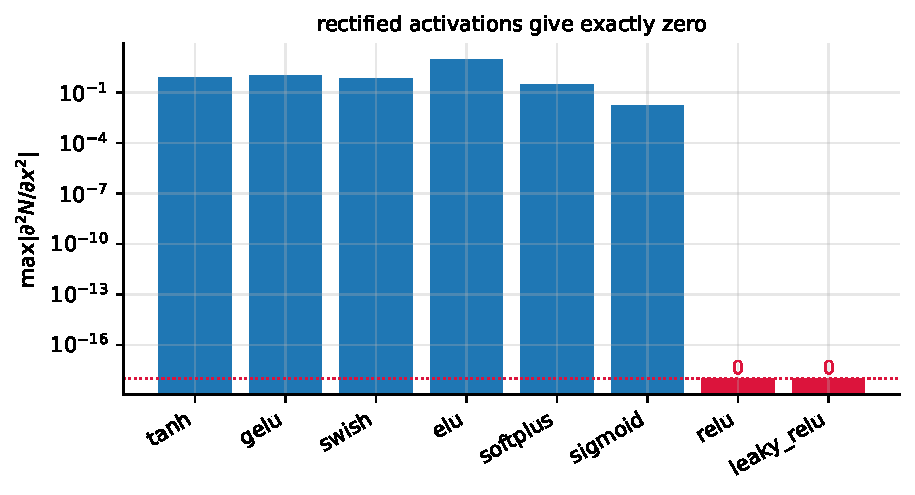
\includegraphics[width=0.84\textwidth]{second_derivative_activations}\par
\scriptsize Book Figure 9.1: $\max|\partial^{2}N/\partial x^{2}|$ of a
freshly initialised $[1,20,20,1]$ network, by activation.
\end{column}
\begin{column}{0.52\textwidth}
\scriptsize
Our own run of the same experiment (\texttt{week42.ipynb}, seed 2026):
\begin{center}
\begin{tabular}{@{}lr@{\qquad}lr@{}}
\toprule
activation & $\max|N''|$ & activation & $\max|N''|$\\
\midrule
tanh & $2.9$ & ELU & $18.9$\\
sigmoid & $0.059$ & GELU & $1.16$\\
softplus & $0.26$ & Swish & $0.72$\\
ReLU & $\mathbf{0}$ & leaky ReLU & $\mathbf{0}$\\
\bottomrule
\end{tabular}
\end{center}
\begin{block}{Not small: identically zero}
\scriptsize
Equation (9.6) needs $f''$.  For the rectified family $f''\equiv0$ wherever
it is defined and $f'$ is piecewise constant, so \emph{every} term of (9.6)
vanishes: a ReLU network has an identically zero second derivative almost
everywhere.  It cannot represent the curvature a second-order equation is
about -- Poisson, diffusion, wave -- and no width or training rescues it.
The smooth activations differ among themselves by two orders of magnitude
and all of them work.  \textbf{Our choice:} $\tanh$ -- smooth, bounded,
$f'=1-f^{2}$ and $f''=-2ff'$ in terms of the function value.  GELU is the
usual default of the PINN literature.
\end{block}
\end{column}
\end{columns}
\end{frame}

\begin{insight}[a ReLU network in a second-order equation: what does the residual report?]
\question{Take the diffusion equation $\partial_tu=\partial_x^{2}u$ and the
physics-informed cost of Part 4, where the network itself is the solution,
$u=N(x,t,P)$, and the equation residual is $L_{\mathrm{PDE}}=\frac1N\sum_i
(\partial_tN-\partial_x^{2}N)^{2}$.  With ReLU hidden units, what is
$\partial_x^{2}N$, what does $L_{\mathrm{PDE}}$ reduce to, how does Adam
minimise it, and what does the trained network look like?  Is the residual
you print at the end a lie?}
\answer{$\partial_x^{2}N\equiv0$ almost everywhere, so
$L_{\mathrm{PDE}}=\frac1N\sum_i(\partial_tN)^{2}$, and the optimiser makes it
zero by making $N$ \emph{independent of $t$}: every weight that multiplies
the $t$ input is driven to zero.  The equation residual is then exactly
zero, on every collocation point, for a solution that does not diffuse at
all -- a ``perfect'' residual and a meaningless answer.  The initial and
boundary terms of the cost fight back (the solution must be $\sin\pi x$ at
$t=0$ and $0$ at the walls, which a $t$-independent $N$ cannot do with
$\partial_x^{2}N=0$ either), so the run ends in a compromise that
satisfies nothing well.  The printed residual is not a lie, it is
\emph{true of the wrong object}: the second derivative the equation asks
for was never in the model.  Hence the rule of Section 9.3: always plot the
residual \emph{and} compare against something -- here the exact solution,
in general a classical method.  A residual that falls suspiciously fast
deserves suspicion.}
\end{insight}

\begin{frame}[fragile]{The code: the week-41 network in \texttt{jax.numpy}, Adam, and \texttt{solve\_de}}
\vspace{-3pt}
\begin{columns}[T]
\begin{column}{0.58\textwidth}
\lstset{basicstyle=\ttfamily\tiny}
\begin{lstlisting}
def network(layers, X, activation="tanh"):
    """The week-41 forward pass in jax.numpy, linear output -> N(x)."""
    f = JAX_ACTIVATIONS[activation]
    a = X
    for l, (W, b) in enumerate(layers):
        z = a @ W + b
        a = f(z) if l < len(layers) - 1 else z
    return a[:, 0]

def d_dxk(fun, k):
    """d fun(layers, X)/d x_k, row by row; nest it for d2/dx_k^2."""
    def wrapped(layers, X):
        def one_row(xk, row):
            return fun(layers, row.at[k].set(xk)[None, :])[0]
        return jax.vmap(jax.grad(one_row), in_axes=(0, 0))(X[:, k], X)
    return wrapped

def adam_minimise(cost_fn, params, n_iter=2000, gamma=1e-2, ...):
    """Adam, Eqs. (4.67)-(4.71), on any nested structure of arrays."""
    @jax.jit
    def step(params, m, v, it):
        c, g = jax.value_and_grad(cost_fn)(params)   # reverse mode, by JAX
        ...                                           # week 38's update, leaf by leaf
        return params, m, v, c
    ...                                               # the loop over iterations

def solve_de(residual, sizes, X, activation="tanh", n_iter=2000, gamma=1e-2, rng=None):
    """Minimise the mean squared residual, Eq. (9.3)."""
    layers = to_jax(create_layers(sizes, activation, rng))   # week 41's initialisation
    cost_fn = lambda layers: jnp.mean(residual(layers, X)**2)
    return adam_minimise(cost_fn, layers, n_iter=n_iter, gamma=gamma)
\end{lstlisting}
\end{column}
\begin{column}{0.4\textwidth}
\begin{block}{What is reused}
\scriptsize
\texttt{create\_layers} with its $1/M_{l-1}$ initialisation; the forward
pass \texttt{a @ W + b} with the linear output, the \texttt{"mse"} head;
the Adam update of week 38 line for line.  \texttt{jax.value\_and\_grad}
replaces our hand-written \texttt{backpropagation}: the residual is an
explicit function of the weights and we \emph{could} derive its gradient
as in Section 8.8, but it now contains the input-derivative recursion as
well, and the derivation carries no insight.  This is the situation
automatic differentiation exists for.
\end{block}
\begin{block}{What is new}
\scriptsize
Two functions per problem -- the \emph{trial solution} (the conditions)
and the \emph{residual} (the equation) -- and \texttt{d\_dxk}: the
derivative of a function of $\bm{X}$ with respect to one input column, one
row at a time (\texttt{jax.grad} of a scalar, vectorised with
\texttt{jax.vmap}).  Everything else is the same five lines for every
equation of this lecture, the PDEs included.  \texttt{jax.jit} compiles
the step once; $3000$ iterations take two seconds.
\end{block}
\end{column}
\end{columns}
\end{frame}

\begin{frame}[fragile]{Exponential decay in code: a trial solution, a residual, one call}
\begin{columns}[T]
\begin{column}{0.58\textwidth}
\lstset{basicstyle=\ttfamily\scriptsize}
\begin{lstlisting}
kappa, g0 = 2.0, 10.0
X = np.linspace(0, 1, 50)[:, None]          # 50 collocation points

def trial_decay(layers, X):                  # Eq. (9.9)
    return g0 + X[:, 0] * network(layers, X, "tanh")

def residual_decay(layers, X):               # Eq. (9.11)
    dg = d_dxk(trial_decay, 0)(layers, X)    # g_t' = N + x dN/dx, by AD
    return dg + kappa * trial_decay(layers, X)

layers, history = solve_de(residual_decay, [1, 40, 40, 1], X, "tanh",
                           n_iter=3000, gamma=2e-2,
                           rng=np.random.default_rng(1))

xx = np.linspace(0, 1, 401)[:, None]         # evaluate anywhere
g = trial_decay(layers, jnp.asarray(xx))
print(np.abs(g - g0*np.exp(-kappa*xx[:, 0])).max())   # 3.1e-03
\end{lstlisting}
\end{column}
\begin{column}{0.4\textwidth}
\begin{block}{Read it as a recipe}
\scriptsize
\begin{enumerate}
  \item Choose collocation points -- any points, no measurements.
  \item Write $g_t$ so that the conditions hold for every $P$ (here
        $g_0+xN$).
  \item Write the residual of the equation in terms of $g_t$ and its
        derivatives, obtained by \texttt{d\_dxk}.
  \item Minimise the mean squared residual with the optimiser of week 38.
  \item Evaluate $g_t$ wherever you like -- and \emph{compare with
        something}.
\end{enumerate}
\end{block}
\scriptsize
Logistic growth: change two lines (the residual, $g_0$).  Poisson: change
the trial solution to $x(1-x)N$ and nest \texttt{d\_dxk} twice.  The
diffusion equation: two input columns.
\end{column}
\end{columns}
\end{frame}

\begin{frame}{Exponential decay, Eqs.~(9.7)--(9.11): the simplest test, and a cautionary one}
\small
\begin{columns}[T]
\begin{column}{0.5\textwidth}
\begin{block}{The equation and the trial solution}
\footnotesize
$g'(x)=-\kappa g(x)$, $g(0)=g_0$; exact $g=g_0e^{-\kappa x}$;
$\kappa=2$, $g_0=10$.  One condition, so $h_1=g_0$ and $h_2=xN$:
\[
  g_t(x,P)=g_0+x\,N(x,P),\qquad
  g_t'=N+x\frac{\partial N}{\partial x}\quad(9.9,\,9.10),
\]
$g_t(0)=g_0$ identically, because the factor $x$ annihilates the network at
the origin.  Residual (9.11): $r=g_t'+\kappa g_t$.
\end{block}
\begin{block}{Result, $[1,40,40,1]$, 50 points, 3000 Adam iterations at $\gamma=0.02$}
\footnotesize
Cost (mean squared residual) $2\times10^{-3}$, maximum error
$3.1\times10^{-3}$ on $[0,1]$ -- relative error $3\times10^{-4}$ of $g_0$.
The book's three seeds give $4.5\times10^{-3}$, $4.1\times10^{-4}$ and
$2.0\times10^{-2}$: accurate, and varying by a factor fifty between runs that
differ only in the initialisation.
\end{block}
\end{column}
\begin{column}{0.48\textwidth}
\includegraphics[width=\textwidth]{week42_ode_cost}\par
\vspace{-3pt}
\begin{block}{A cautionary result (Section 9.3)}
\scriptsize
Two hidden layers of \emph{twenty} units at $\gamma=0.01$: the cost falls to
$31.9$ and stays there -- after $3000$ iterations, after $10\,000$, at
$\gamma=0.02$ -- and the solution is wrong by $1.83$, eighteen per cent.
Forty units, or $\gamma=0.05$, escape at once.  This is the non-convexity of
Section 8.7 in the flesh: a local minimum where the gradient is
\emph{genuinely} zero.  A classical solver converges or reports failure; a
network can converge confidently to the wrong answer.  \emph{Always plot the
residual, always compare against something.}
\end{block}
\end{column}
\end{columns}
\end{frame}

\begin{frame}{Logistic growth, Eqs.~(9.12)--(9.14), against forward Euler}
\small
\begin{columns}[T]
\begin{column}{0.5\textwidth}
\begin{block}{A non-linear equation}
\footnotesize
$g'(t)=\alpha g(t)\bigl(A-g(t)\bigr)$, $g(0)=g_0$; exact
$g=Ag_0/\bigl(g_0+(A-g_0)e^{-\alpha At}\bigr)$; $\alpha=2$, $A=1$,
$g_0=1.2$ -- the population starts above the carrying capacity and decays
towards it.  Same condition, same trial solution $g_t=g_0+tN$; only the
residual changes: $r=g_t'-\alpha g_t(A-g_t)$.  Non-linearity costs nothing
in this framework.
\end{block}
\begin{block}{The classical competitor}
\footnotesize
Forward Euler, $g_{i+1}=g_i+\Delta t\,\alpha g_i(A-g_i)$, error
$\mathcal{O}(\Delta t)$:
\begin{center}
\scriptsize
\begin{tabular}{@{}lr@{}}
\toprule
method & max error on $[0,1]$\\
\midrule
Euler, 10 steps ($\Delta t=0.1$) & $9.9\times10^{-3}$\\
Euler, 20 steps & $4.7\times10^{-3}$\\
Euler, 50 steps & $1.8\times10^{-3}$\\
Euler, 100 steps & $8.9\times10^{-4}$\\
network, 50 points & $\mathbf{1.2\times10^{-4}}$\\
\bottomrule
\end{tabular}
\end{center}
\end{block}
\end{column}
\begin{column}{0.48\textwidth}
\begin{block}{Reading the table honestly}
\scriptsize
The Euler errors halve when the step halves -- first order, as it should
be -- and the network with fifty points is ten times more accurate than
Euler with fifty steps, and has no systematic lag (Figure (b) of the next
frame).  That comparison flatters the network.  Euler took microseconds; the
network took $3000$ Adam iterations.  A second-order Runge--Kutta scheme
with fifty steps would beat the network at a cost still negligible beside
it.  The network's case lies elsewhere (Section 9.9, at the end of Part 3).
\end{block}
\begin{block}{Our numbers}
\scriptsize
$[1,40,40,1]$, $3000$ iterations at $\gamma=0.02$, seed 1: final cost
$1.1\times10^{-6}$, max error $1.15\times10^{-4}$ -- the book's number to
the digit, because the construction is deterministic once the seed is.
\end{block}
\end{column}
\end{columns}
\end{frame}

\begin{frame}{The Poisson equation (9.15)--(9.19) against finite differences}
\small
\begin{columns}[T]
\begin{column}{0.5\textwidth}
\begin{block}{The equation and the trial solution}
\scriptsize
$-g''(x)=f(x)$ on $(0,1)$, $g(0)=g(1)=0$, with $f=(3x+x^{2})e^{x}$ and the
exact $g=x(1-x)e^{x}$.  Two conditions:
\[
  g_t(x,P)=x(1-x)\,N(x,P)\quad(9.18),
\]
zero at both ends for every $P$, $h_1\equiv0$.  By the product rule (9.19)
$g_t''=-2N+2(1-2x)N'+x(1-x)N''$: all of $N,N',N''$ appear, the first example
that fails outright with ReLU.  Residual $r=-g_t''-f$, \texttt{d\_dxk}
nested twice.
\end{block}
\begin{block}{The classical competitor, Eqs.~(9.20)--(9.22)}
\scriptsize
Taylor-expand $u(x_i\pm\Delta x)$ and add: the odd terms cancel,
$u_i''=(u_{i+1}-2u_i+u_{i-1})/\Delta x^{2}+\mathcal{O}(\Delta x^{2})$, and
the equation becomes a tridiagonal system with the discrete Laplacian,
solved in $\mathcal{O}(n)$ operations (LU, Section 1.14).
\end{block}
\end{column}
\begin{column}{0.48\textwidth}
\begin{center}
\scriptsize
\begin{tabular}{@{}lr@{}}
\toprule
method & max error\\
\midrule
FD, 10 intervals ($\Delta x=0.1$) & $2.2\times10^{-3}$\\
FD, 20 intervals & $5.4\times10^{-4}$\\
FD, 50 intervals & $8.7\times10^{-5}$\\
FD, 100 intervals & $2.2\times10^{-5}$\\
network $[1,30,30,1]$, 60 points, seed 1 & $\mathbf{1.2\times10^{-5}}$\\
same, seed 2, 4000 iterations & $2.1\times10^{-2}$\\
same, seed 2, 8000 iterations & $5.7\times10^{-6}$\\
\bottomrule
\end{tabular}
\end{center}
\begin{block}{Reading it}
\scriptsize
The finite-difference error falls by four when $\Delta x$ halves --
$\mathcal{O}(\Delta x^{2})$ confirmed -- and the converged network sits at
the hundred-interval level with sixty points: comparable accuracy per
point, one tridiagonal solve against four thousand Adam iterations.  The
two seeds: same architecture, same $\gamma$, one run converged at $4000$
iterations, the other sat at a cost of $0.027$ until $8000$ -- and on a
different machine (Apple silicon, another JAX version) seed 2 converges at
$4000$ while the decay error becomes $1.2\times10^{-2}$: rounding decides
the path through a non-convex landscape.  Here the classical method wins
decisively; the example is a \emph{verification}.
\end{block}
\end{column}
\end{columns}
\end{frame}

\begin{frame}{The three ordinary differential equations (\texttt{week42\_ode.pdf})}
\centering
\includegraphics[width=0.98\textwidth]{week42_ode}\par
\vspace{-4pt}
\raggedright\scriptsize
The network solution (circles, every sixteenth of $401$ evaluation points)
against the exact solution (line), with the classical competitor at its
coarsest setting.  \textbf{(a)} Decay: max error $3.1\times10^{-3}$ on a
solution of size $10$.  \textbf{(b)} Logistic growth: forward Euler with ten
steps lags visibly behind the curve, the $\mathcal{O}(\Delta t)$ error of a
first-order scheme; the network has no step and no lag.  \textbf{(c)}
Poisson: finite differences with ten intervals, error $2\times10^{-3}$, and
the network at $10^{-5}$.  In every panel the collocation points were the
$50$ or $60$ equally spaced points of the training, and the network is
evaluated \emph{between} them -- it returns a function, not a table.
\end{frame}

\begin{insight}[design the trial solution]
\question{The trial solution carries the conditions, and the factor in front
of $N$ must vanish wherever a condition is imposed.  Write $g_t$ for (i)
$g(0)=g_0$ \emph{and} $g'(0)=v_0$ (a second-order initial-value problem);
(ii) $g(0)=a$, $g(1)=b$ with $a,b\neq0$; (iii) $g(0)=0$ and $g'(1)=0$ (a
Neumann condition at the right end).  Which of the three is awkward, and
why?}
\answer{(i) $g_t=g_0+v_0x+x^{2}N$: at $x=0$ the value is $g_0$; the
derivative $v_0+2xN+x^{2}N'$ is $v_0$ at $x=0$ because every term with $N$
carries at least one factor $x$ -- the $t^{2}$ device of the wave equation,
Eq.~(9.33).  (ii) $g_t=a+(b-a)x+x(1-x)N$: $h_1$ is the straight line through
the two boundary values, $h_2$ vanishes at both ends.  (iii) is the awkward
one: $h_2$ must vanish at $x=0$ and have zero \emph{derivative} at $x=1$,
and no prefactor alone does it -- $x(2-x)N$ has derivative $N'(1)$ at
$x=1$.  One has to subtract what the network does at the boundary, e.g.\
$g_t=xN(x)-\tfrac12x^{2}\bigl[N(1)+N'(1)\bigr]$, whose derivative at $x=1$
is $N(1)+N'(1)-N(1)-N'(1)=0$: doable here, a different formula for every
geometry and every type of condition, and impossible on an L-shaped domain.
That is the straitjacket Section 9.10
removes, at a price we shall measure.}
\end{insight}

%% ====================================================================
%% Part 3: the diffusion equation (Sections 9.6-9.7)
%% ====================================================================

\begin{frame}{Partial differential equations: the same strategy, two inputs (9.6)}
\small
\begin{columns}[T]
\begin{column}{0.48\textwidth}
\begin{block}{Nothing changes but the input layer}
\footnotesize
$f\bigl(x_1,\dots,x_N,\partial g/\partial x_1,\dots,\partial^{n}g/\partial
x_N^{n}\bigr)=0$ (9.23), the trial solution
$g_t=h_1(\bm{x})+h_2(\bm{x},N(\bm{x},P))$ (9.24), and the cost (9.25) the
mean squared residual over $M$ collocation points $\bm{x}_i$ forming the
rows of $\bm{X}$.  The network now has $N$ input nodes -- \texttt{sizes =
[2, 30, 30, 1]} for $(x,t)$ -- and that is the \emph{only} change.  Which is
the point of having built it generally.
\end{block}
\begin{block}{The derivatives}
\footnotesize
By nested AD on the trial solution, one coordinate at a time:
\texttt{d\_dxk(g, 1)} is $\partial_tg$, \texttt{d\_dxk(d\_dxk(g, 0), 0)}
is $\partial_x^{2}g$ -- and the parameter gradient of the whole thing comes
from \texttt{jax.value\_and\_grad}, as before.
\end{block}
\end{column}
\begin{column}{0.5\textwidth}
\begin{block}{The diffusion equation, Eqs.~(9.26)--(9.28)}
\footnotesize
\[
  \frac{\partial g(x,t)}{\partial t}=\frac{\partial^{2}g(x,t)}{\partial x^{2}},
\]
with $g(0,t)=g(1,t)=0$ and $g(x,0)=u(x)=\sin\pi x$; exact solution
$g=e^{-\pi^{2}t}\sin\pi x$, which decays by $e^{-\pi^{2}}\approx5\times10^{-5}$
over a unit of time.
\end{block}
\begin{block}{Three conditions, one trial solution, Eq.~(9.29)}
\footnotesize
\[
  \boxed{\;g_t(x,t,P)=(1-t)\,u(x)+x(1-x)\,t\,N(x,t,P)\;}
\]
At $t=0$ the second term vanishes and the first is $u(x)$; at $x=0$ and
$x=1$ the factor $x(1-x)$ kills the network and $u(0)=u(1)=0$ kills the
first term.  All three hold identically, for every $P$.
\end{block}
\end{column}
\end{columns}
\end{frame}

\begin{frame}[fragile]{The diffusion equation in code}
\begin{columns}[T]
\begin{column}{0.6\textwidth}
\lstset{basicstyle=\ttfamily\scriptsize}
\begin{lstlisting}
def trial_diffusion(layers, X):                   # Eq. (9.29)
    x, t = X[:, 0], X[:, 1]
    return ((1 - t)*jnp.sin(jnp.pi*x)
            + x*(1 - x)*t*network(layers, X, "tanh"))

def residual_diffusion(layers, X):                # Eq. (9.26)
    g_t  = d_dxk(trial_diffusion, 1)
    g_xx = d_dxk(d_dxk(trial_diffusion, 0), 0)
    return g_t(layers, X) - g_xx(layers, X)

xs, ts = np.linspace(0, 1, 20), np.linspace(0, 1, 20)
Xg, Tg = np.meshgrid(xs, ts, indexing="ij")
X = np.column_stack([Xg.ravel(), Tg.ravel()])     # 400 points
layers, history = solve_de(residual_diffusion, [2, 30, 30, 1], X,
                           "tanh", n_iter=800, gamma=1e-2,
                           rng=np.random.default_rng(1))
\end{lstlisting}
\end{column}
\begin{column}{0.38\textwidth}
\begin{block}{Count the changes}
\scriptsize
Two input columns; a trial solution with three conditions built in; a
residual with one first and one second derivative.  \texttt{solve\_de},
\texttt{network}, \texttt{d\_dxk} and Adam are untouched: $1021$
parameters, $400$ collocation points, $800$ iterations, three seconds.
\end{block}
\begin{block}{What to look at}
\scriptsize
Not the cost alone.  Evaluate on a finer grid ($101\times101$), compare
with the exact solution, slice by time -- and check the three edges where
the conditions were imposed.
\end{block}
\end{column}
\end{columns}
\end{frame}

\begin{frame}{The diffusion equation solved (\texttt{week42\_diffusion.pdf})}
\centering
\includegraphics[width=0.98\textwidth]{week42_diffusion}\par
\vspace{-4pt}
\raggedright\scriptsize
$[2,30,30,1]$, tanh, $800$ Adam iterations at $\gamma=0.01$ (three seconds),
evaluated on a $101\times101$ grid.  \textbf{(a)} Time slices: the network
(circles) on the exact curves; the squares are an explicit finite-difference
scheme, $u_i^{n+1}=u_i^{n}+\alpha(u_{i+1}^{n}-2u_i^{n}+u_{i-1}^{n})$ with
$\Delta x=0.05$ and $\alpha=\Delta t/\Delta x^{2}=\frac12$, the largest
stable step -- $800$ steps of $\Delta t=0.00125$ to reach $t=1$.
\textbf{(b)} The absolute error, largest ($1.0\times10^{-2}$) at
$x=0.42$, $t=0.05$ where the solution changes fastest, and \emph{exactly
zero} along $t=0$, $x=0$ and $x=1$: not small, zero to machine precision,
at every stage of training, because (9.29) satisfies the conditions
identically.  RMSE $1.8\times10^{-3}$; $4000$ iterations do not improve it
($1.09\times10^{-2}$, $1.7\times10^{-3}$).  \textbf{(c)} The maximum error
over $x$ against $t$: the network's stays near $10^{-3}$ while the solution
(dotted) decays by four orders of magnitude; the finite-difference error
decays \emph{with} the solution.  Max error $1.5\times10^{-3}$ for the
scheme, in milliseconds.
\end{frame}

\begin{insight}[an absolute error that does not decay]
\question{Panel (c): at $t=1$ the exact solution is $e^{-\pi^{2}}\approx
5\times10^{-5}$ and the network's error is still about $10^{-3}$ -- the
\emph{relative} error exceeds one, while the finite-difference solution
tracks the decay.  Why does the cost (9.25) not care?  What does
$\tfrac1M\sum_i r_i^{2}$ weight, and what would you change -- in the
collocation points, in the residual, or in the trial solution -- to get the
late times right?}
\answer{The cost is a \emph{mean of squared absolute residuals} over
collocation points spread uniformly over $[0,1]^{2}$.  Where the solution is
$10^{-4}$ the residual of a network that returns $10^{-3}$ is $10^{-3}$ --
invisible next to the residuals of $10^{-1}$ near $t=0$ where the solution
moves fast.  Adam spends its effort where the squared residual is large, and
that is early times.  Remedies, in increasing order of knowledge used:
(i) more collocation points at late times, or weights $w_i$ on the
residuals -- cheap, and the beginning of the weighting problem of Part 4;
(ii) a relative residual, $r_i/(|g_t|+\epsilon)$, or the equation for
$\ln g$; (iii) build the decay into the trial solution,
$g_t=e^{-\pi^{2}t}\bigl[\sin\pi x+x(1-x)tN\bigr]$ -- which is cheating here,
since $e^{-\pi^{2}t}$ is the answer, but is exactly what one does when the
asymptotics are known and the shape is not.  Information put into the
ansatz is free and exact; information requested through the cost is paid
for in optimisation effort -- the theme of Part 4.}
\end{insight}

\begin{frame}{When is this worth doing? (Section 9.9)}
\small
\begin{columns}[T]
\begin{column}{0.5\textwidth}
\begin{block}{The comparisons were deliberately unflattering}
\scriptsize
Runge--Kutta beats the network on the logistic equation, a tridiagonal
solve on the Poisson equation, the explicit scheme on the diffusion
equation -- all of them by orders of magnitude in time.  For textbook
problems in one or two dimensions classical numerical analysis wins
comfortably.  Any presentation of this material that omits the comparison
is selling something.
\end{block}
\begin{block}{Machine-learning connection (Section 9.9)}
\scriptsize
The cost (9.25) is regression in disguise: the residual is the target, the
collocation points are the data.  Everything of Chapters 4 and 8 applies --
and so do the difficulties: non-convexity (the $31.9$ run), conditioning
(Section 4.5), the activation deciding whether the derivatives exist, and no
analogue of the theorem that says a scheme is $\mathcal{O}(\Delta x^{2})$.
We trade guarantees for flexibility.
\end{block}
\end{column}
\begin{column}{0.48\textwidth}
\begin{block}{Where the flexibility is needed}
\scriptsize
\begin{itemize}
  \item \textbf{High dimension.}  A mesh grows exponentially with the
        dimension; collocation points can be sampled, and the cost grows with
        the number of \emph{parameters}.  Hamilton--Jacobi--Bellman, the
        many-body Schr\"odinger equation: meshes are impossible, networks
        are not.
  \item \textbf{Complicated geometry.}  No mesh to build; sample the domain.
  \item \textbf{The solution as a function.}  Evaluate, differentiate,
        compose anywhere -- no interpolation step.  Both networks of this
        lecture were trained on $20\times20$ points and evaluated on
        $101\times101$.
  \item \textbf{Inverse problems and data assimilation.}  An unknown
        coefficient, a few measurements: add a data-misfit term and optimise
        over the coefficient alongside the weights.  Unchanged machinery; for
        a classical solver an adjoint calculation and an outer loop.  This is
        what ``physics-informed'' usually means -- Part 4.
\end{itemize}
\end{block}
\end{column}
\end{columns}
\end{frame}

%% ====================================================================
%% Part 4: physics-informed neural networks (Section 9.10)
%% ====================================================================

\begin{frame}{Physics-informed neural networks: drop the trial solution (9.10)}
\small
\begin{columns}[T]
\begin{column}{0.48\textwidth}
\begin{block}{The straitjacket}
\scriptsize
$h_1$ and $h_2$ must be written by hand for every problem.  For the unit box
with homogeneous Dirichlet conditions $x(1-x)t$ does it; for a curved
boundary, a Neumann or Robin condition, a coupled system, an L-shaped domain
or an annulus, it ranges from tedious to impossible (Pause and think 4).
Raissi, Perdikaris and Karniadakis (2019) coined the name; this section
follows a tutorial written for the course by F.\ Nys{\ae}ter, O.\ Fausko
and K.\ Liodden.
\end{block}
\begin{block}{The opposite view, Eq.~(9.34)}
\scriptsize
Let the network itself be the solution, $u(\bm{x})\approx N(\bm{x},P)$, with
no scaffolding -- and \emph{demand} the conditions of the optimiser instead,
one least-squares penalty each.  Hard constraints become \emph{soft} ones,
satisfied approximately at the optimum.  Four point sets instead of one:
$N_{\mathrm{pde}}$ collocation points in the interior, $N_{\mathrm{ic}}$ on
$t=0$, $N_{\mathrm{bc}}$ on each of $x=0$ and $x=1$.
\end{block}
\end{column}
\begin{column}{0.5\textwidth}
\begin{block}{The composite cost for the diffusion problem, Eqs.~(9.35)--(9.38)}
\scriptsize
\begin{align*}
  L_{\mathrm{PDE}}&=\tfrac{1}{N_{\mathrm{pde}}}\textstyle\sum_i\bigl(\partial_tN-\partial_x^{2}N\bigr)^{2}_{(x_i,t_i)},\\
  L_{\mathrm{IC}}&=\tfrac{1}{N_{\mathrm{ic}}}\textstyle\sum_i\bigl(N(x_i,0,P)-u(x_i)\bigr)^{2},\\
  L_{\mathrm{BC}}&=\tfrac{1}{N_{\mathrm{bc}}}\textstyle\sum_iN(0,t_i,P)^{2}
  +\tfrac{1}{N_{\mathrm{bc}}}\sum_iN(1,t_i,P)^{2},\\
  &\boxed{\;L_{\mathrm{total}}=L_{\mathrm{PDE}}+\lambda_{\mathrm{IC}}L_{\mathrm{IC}}+\lambda_{\mathrm{BC}}L_{\mathrm{BC}}\;}
\end{align*}
$L_{\mathrm{PDE}}$ is exactly the cost we have minimised all along, with $N$
in place of $g_t$.  The weights $\lambda$ play the role of the penalty
parameters of Ridge regression (Section 3.8): how much we care about one
group of residuals relative to another.  Nothing in Chapters 4 and 8 changes.
\end{block}
\end{column}
\end{columns}
\end{frame}

\begin{frame}[fragile]{The code: one point set becomes several, and the cost acquires weights}
\vspace{-3pt}
\begin{columns}[T]
\begin{column}{0.58\textwidth}
\lstset{basicstyle=\ttfamily\tiny}
\begin{lstlisting}
def pinn_solve(terms, sizes, activation="tanh", n_iter=2000, gamma=1e-2, rng=None, ...):
    """terms: list of (name, weight, residual_fn, points), Eq. (9.38)."""
    layers = to_jax(create_layers(sizes, activation, rng))
    def cost_fn(layers):
        return sum(w*jnp.mean(residual(layers, Xk)**2) for _, w, residual, Xk in terms)
    return adam_minimise(cost_fn, layers, n_iter=n_iter, gamma=gamma, ...)

xs, ts = np.linspace(0, 1, 20), np.linspace(0, 1, 20)
Xi, Ti = np.meshgrid(xs[1:-1], ts[1:-1], indexing="ij")     # interior only
X_col = np.column_stack([Xi.ravel(), Ti.ravel()])           # 324 points
X_ic  = np.column_stack([xs, np.zeros(20)])                 # t = 0
X_l   = np.column_stack([np.zeros(20), ts])                 # x = 0
X_r   = np.column_stack([np.ones(20),  ts])                 # x = 1

def u_net(layers, X): return network(layers, X, "tanh")     # Eq. (9.34)
u_t  = d_dxk(u_net, 1)
u_xx = d_dxk(d_dxk(u_net, 0), 0)

def r_pde(layers, X): return u_t(layers, X) - u_xx(layers, X)       # (9.35)
def r_ic(layers, X):  return u_net(layers, X) - jnp.sin(jnp.pi*X[:, 0])  # (9.36)
def r_bc(layers, X):  return u_net(layers, X)                        # (9.37)

terms = [("pde", 1.0, r_pde, X_col), ("ic", 10.0, r_ic, X_ic),
         ("bcL", 10.0, r_bc, X_l),   ("bcR", 10.0, r_bc, X_r)]
layers, history = pinn_solve(terms, [2, 30, 30, 1], "tanh", n_iter=4000,
                             gamma=1e-2, rng=np.random.default_rng(1))
\end{lstlisting}
\end{column}
\begin{column}{0.4\textwidth}
\begin{block}{The whole difference, at the level of code}
\scriptsize
\texttt{solve\_de} took one residual on one point set;
\texttt{pinn\_solve} takes a list of them with weights.  The network,
\texttt{d\_dxk}, the initialisation and the optimiser are the ones of Part
2.  A new condition is a new line in \texttt{terms}: a Neumann condition
$\partial_xu=q$ is \texttt{("neu", 10.0, lambda L, X: u\_x(L, X) - q, X\_r)},
and an initial velocity for the wave equation is \texttt{u\_t} on
\texttt{X\_ic} -- the one condition that took thought in the trial solution
takes one line here.
\end{block}
\begin{block}{Why the interior points exclude the boundaries}
\scriptsize
A point carrying both the equation residual and a boundary residual is asked
two things at once, and the two requests compete.  $324$ interior points,
$20$ on each edge.
\end{block}
\end{column}
\end{columns}
\end{frame}

\begin{frame}{Hard against soft on identical ground (Table 9.1)}
\scriptsize
Same $[2,30,30,1]$ network, same $\tanh$, same Adam at $\gamma=0.01$, same
seed; errors on the $101\times101$ evaluation grid against (9.28).
\begin{center}
\setlength{\tabcolsep}{5pt}
\begin{tabular}{@{}lrccc@{}}
\toprule
Formulation & Iterations & max error & RMSE & error at $t=0$\\
\midrule
Hard, Eq.~(9.29) & 800 & $1.04\times10^{-2}$ & $1.79\times10^{-3}$ & $0$ exactly\\
Hard, Eq.~(9.29) & 4000 & $1.09\times10^{-2}$ & $1.68\times10^{-3}$ & $0$ exactly\\
Soft, $\lambda=1$ & 800 & $2.93\times10^{-2}$ & $4.12\times10^{-3}$ & $2.93\times10^{-2}$\\
Soft, $\lambda=10$ & 800 & $3.51\times10^{-2}$ & $1.35\times10^{-2}$ & $3.51\times10^{-2}$\\
Soft, $\lambda=100$ & 800 & $4.00\times10^{-2}$ & $7.06\times10^{-3}$ & $1.48\times10^{-2}$\\
Soft, $\lambda=10$ & 4000 & $3.18\times10^{-2}$ & $6.45\times10^{-3}$ & $6.29\times10^{-3}$\\
\bottomrule
\end{tabular}
\end{center}
\begin{columns}[T]
\begin{column}{0.5\textwidth}
\begin{block}{The hard formulation wins on every measure}
\scriptsize
RMSE three to four times smaller, and the error at $t=0$ not merely smaller
but zero.  Five times more training does not close the gap: the soft
solution's largest error is still $3\times10^{-2}$ after $4000$ iterations,
at $x=0.48$, $t=0.04$, where the solution decays fastest.  \emph{On a
problem where a trial solution can be constructed, constructing it is
better.}  Information built into the ansatz is free and exact; information
supplied through the cost is paid for in optimisation effort and is never
exact.
\end{block}
\end{column}
\begin{column}{0.48\textwidth}
\begin{block}{The weights are a real difficulty}
\scriptsize
$\lambda$ from $1$ to $10$ changes little; $100$ makes everything worse --
the optimiser spends its capacity on the edges and $L_{\mathrm{PDE}}$ rises
tenfold ($0.0009\to0.010$).  There is a best $\lambda$, it is
problem-dependent, and we found it by trying three values.  The reason is
conditioning (Section 4.5): the four terms have gradients of very different
sizes -- $L_{\mathrm{PDE}}$ carries $\bm{W}^{2}$ through the second
derivative, $L_{\mathrm{IC}}$ the value alone -- and one $\gamma$ must
serve all.  Choosing the weights automatically is an open research problem.
\end{block}
\end{column}
\end{columns}
\end{frame}

\begin{frame}{Soft constraints at work (\texttt{week42\_pinn.pdf})}
\centering
\includegraphics[width=0.98\textwidth]{week42_pinn}\par
\vspace{-4pt}
\raggedright\scriptsize
$\lambda=10$, $4000$ iterations.  \textbf{(a)} The four terms of
Eq.~(9.38), unweighted, during training: they descend at different rates
and by different amounts, and the spikes every few hundred iterations are
the terms trading against one another -- an edge term jumps by two orders
of magnitude when the equation term takes a step the edges do not like.
\textbf{(b)} The error of the converged solution: largest in the
fast-decaying region near $t=0$, not on the boundaries, and \emph{nowhere}
zero.  \textbf{(c)} The initial condition: the soft formulation misses
$\sin\pi x$ by up to $6\times10^{-3}$ after $4000$ iterations; the hard
formulation of Eq.~(9.29) satisfies it identically -- the blue line is not
small, it is zero, and it would be zero for an untrained network.
\end{frame}

\begin{frame}[fragile]{So why soft constraints at all?  The inverse problem, Eqs.~(9.39)--(9.40)}
\begin{columns}[T]
\begin{column}{0.5\textwidth}
\begin{block}{An unknown coefficient and forty measurements}
\scriptsize
$\partial_tu=D\,\partial_x^{2}u$ with $D$ \emph{unknown}, and instead of
initial and boundary conditions a handful of noisy observations
$\{(\bm{x}_i,y_i)\}$ of the solution at scattered points.  Minimise, over
the weights \emph{and} $D$ together,
\begin{align*}
  L(P,D)&=\frac{1}{N_{\mathrm{pde}}}\sum_i\Bigl(\partial_tN-D\,\partial_x^{2}N\Bigr)^{2}_i\\
  &\quad+\lambda_{\mathrm{data}}\frac{1}{N_{\mathrm{data}}}\sum_i\bigl(N(\bm{x}_i,P)-y_i\bigr)^{2}.
\end{align*}
No initial condition, no boundary condition: the data replace them.  A trial
solution cannot even be written down -- the soft formulation is not merely
convenient, it is the only one available.  For a classical solver this is
an outer optimisation loop around the solver, with an adjoint equation
derived by hand for the problem at hand.
\end{block}
\end{column}
\begin{column}{0.48\textwidth}
\lstset{basicstyle=\ttfamily\tiny}
\begin{lstlisting}
rng = np.random.default_rng(3)                  # the "measurements"
X_obs = np.column_stack([rng.uniform(0, 1, 40), rng.uniform(0, 1, 40)])
y_obs = np.exp(-0.5*np.pi**2*X_obs[:, 1])*np.sin(np.pi*X_obs[:, 0]) \
        + rng.normal(0, 0.01, 40)

params = (to_jax(create_layers([2, 30, 30, 1], "tanh",
                               np.random.default_rng(1))),
          jnp.array(D0))                        # the weights, and D

def cost_fn(params):
    layers, D = params   # the only line that knows this is an inverse problem
    return (jnp.mean((u_t(layers, X_col) - D*u_xx(layers, X_col))**2)
            + 10.0*jnp.mean((u_net(layers, X_obs) - y_obs)**2))

params, history = adam_minimise(cost_fn, params, n_iter=3000, gamma=1e-2)
\end{lstlisting}
\begin{block}{One more leaf of the parameter tree}
\scriptsize
Adam of week 38 does not care what a parameter \emph{is}: $D$ gets its own
first and second moment and its own step, like every weight.  Seven lines
beyond the forward problem.
\end{block}
\end{column}
\end{columns}
\end{frame}

\begin{frame}{Recovering $D$ from forty noisy points (\texttt{week42\_pinn\_inverse.pdf})}
\begin{columns}[T]
\begin{column}{0.62\textwidth}
\includegraphics[width=\textwidth]{week42_pinn_inverse}\par
\vspace{-3pt}
\scriptsize
$D_{\mathrm{true}}=0.5$, forty observations from the exact solution with
Gaussian noise of standard deviation $0.01$, seed 3; $324$ interior
collocation points.  \textbf{(a)} Three starting values -- $2.0$, four
times too large, $1.0$ and $0.1$ -- converge to the same $D\approx0.513$
within $1500$ iterations.  \textbf{(b)} The recovered solution (solid)
against the exact one (dashed) at three times, with the observations
coloured by the time they were taken; the visible gap at $t=0.05$ is the
three per cent error in $D$.
\end{column}
\begin{column}{0.36\textwidth}
\begin{center}
\scriptsize
\begin{tabular}{@{}lrr@{}}
\toprule
 & $D$ & rel.\ error\\
\midrule
$D_0=2.0$ & $0.5133$ & $2.7\%$\\
$D_0=1.0$ & $0.5148$ & $3.0\%$\\
$D_0=0.1$ & $0.5124$ & $2.5\%$\\
noise $0$, $D_0=2$ & $0.4762$ & $4.8\%$\\
noise $0.05$, $D_0=2$ & $0.6903$ & $38\%$\\
\bottomrule
\end{tabular}
\end{center}
\begin{block}{Not to be oversold}
\scriptsize
The first two noise rows differ by less than the seed-to-seed scatter and
are the same result.  The third is not: five per cent noise on the
observations gives thirty-eight per cent error in $D$.  Inverse problems
are ill-posed; the sensitivity belongs to the problem, not to the method.
\end{block}
\end{column}
\end{columns}
\end{frame}

\begin{insight}[forty points, no conditions, three per cent -- and then thirty-eight]
\question{Equation (9.40) has no initial and no boundary term, yet the
network recovered $D$ to three per cent from forty noisy points and
reproduced the solution in Figure (b).  What supplied the missing
conditions?  Why does the recovered $D$ degrade from $3\%$ to $38\%$ when
the noise goes from $0.01$ to $0.05$ -- is that the method's fault, and
what should a report of ``$D=0.513$'' have come with?}
\answer{The forty observations, together with the equation.  The equation
propagates each measurement through space and time -- a value at $(x_i,t_i)$
constrains the solution everywhere the equation connects it to -- and forty
points scattered over the domain pin down a solution of the heat equation
with a single free parameter.  Conditions are information, and data are
information; the cost only counts residuals.  The collapse at $5\%$ noise is
\emph{not} the method's fault: an inverse problem is ill-posed, the map
from data to $D$ amplifies noise, and a classical adjoint-based inversion
on the same forty points would face the same amplification.  Recovering a
parameter from data is a \emph{statistical estimation} problem, Chapter 2
applies, and a single number without an error estimate is not a result:
bootstrap the observations (week 36), or vary the seed, and report
$D=0.51\pm0.02$ -- or, at $5\%$ noise, admit that forty points do not
determine $D$ to better than a factor of two.}
\end{insight}

\begin{frame}{Soft or hard?  (Section 9.10)}
\small
\begin{columns}[T]
\begin{column}{0.52\textwidth}
\begin{block}{Two points on a scale, not rivals}
\footnotesize
\begin{itemize}
  \item If a trial solution can be constructed, construct it: the conditions
        hold exactly, the cost has one term, there are no weights to tune,
        and Table 9.1 shows the accuracy that buys.
  \item If the geometry is awkward, the conditions involve derivatives or
        mixed terms, or the equations are coupled, use soft constraints.  The
        loss of accuracy is real but bounded; the alternative may be no
        method at all.
  \item If parameters of the equation are unknown and data are available,
        soft constraints are the only option, and extremely convenient.
  \item Mix them: a trial solution for the boundary conditions, a penalty
        for an initial condition -- often the best of the three.
\end{itemize}
\end{block}
\end{column}
\begin{column}{0.46\textwidth}
\begin{block}{The wave equation, in one line (Sections 9.8, 9.10)}
\footnotesize
$\partial_t^{2}g=c^{2}\partial_x^{2}g$ needs the initial velocity too.
Hard: replace $t$ by $t^{2}$ in the trial solution, Eq.~(9.33) -- a device
that must be rethought if $v(x)\neq0$.  Soft: \texttt{("iv", 10.0, u\_t,
X\_ic)}, one line.  Accuracy after $4000$ iterations: hard
$4.8\times10^{-4}$, soft $8.7\times10^{-3}$, eighteen times apart, because
the standing wave never decays and the boundary terms compete for the whole
of training.
\end{block}
\begin{block}{Trained on $20\times20$, evaluated on $101\times101$}
\footnotesize
Both formulations return a differentiable function valid everywhere in the
domain -- not interpolation in the finite-difference sense, but evaluation
of a closed form.  It is one thing the method genuinely does better than a
grid.
\end{block}
\end{column}
\end{columns}
\end{frame}

\begin{frame}{Where this is going: tomorrow, Project 2, next week}
\small
\begin{columns}[T]
\begin{column}{0.5\textwidth}
\begin{block}{Tomorrow: one case, the backward pass}
\footnotesize
Your questions on today, then the structure of this week's exercises: the
gradient of one layer by hand with every shape written down, two layers,
the loop of Eqs.~(8.65)--(8.68) for any depth, the batched version, each
step checked against \texttt{jax.grad} -- in \texttt{week42tuesday.ipynb}
on a problem of our own, so that you do it once with us and once alone in
\texttt{exercisesweek42.ipynb}.  Deadline \textbf{Friday October 16};
declare your use of LLMs.
\end{block}
\begin{block}{Next Monday, week 43}
\footnotesize
Convolutional neural networks (Chapter 10): keeping the spatial structure
that we threw away when we flattened $28\times28$ into $784$ -- the reason
the $4\to9$ and $7\to2$ confusions of week 41 survive a dense network and
do not survive a convolutional one.
\end{block}
\end{column}
\begin{column}{0.48\textwidth}
\begin{block}{Project 2 (deadline November 6)}
\footnotesize
Your own \texttt{feed\_forward}, \texttt{backpropagation} and
\texttt{train} -- exactly the code of the first half hour -- on the Runge
data and on the full MNIST set, against OLS/Ridge and logistic regression,
with the optimisers of week 38, the resampling of week 36, a gradient check
and a confusion matrix.  Everything of Part 1 is a building block; the
differential equations of Parts 2--4 are not part of the project, but the
code is yours if you want a differential equation as your own data set.
\end{block}
\begin{block}{Reading}
\footnotesize
Chapter 9, Sections 9.1--9.7 and 9.9--9.10; the exercises of Section 9.13
repeat Part 2 with GELU, Swish and the sigmoid, reproduce the local minimum,
and add the wave equation with a non-zero initial velocity.
\end{block}
\end{column}
\end{columns}
\end{frame}

%% ====================================================================
%% Summary
%% ====================================================================

\begin{frame}{Summary of week 42}
\footnotesize
\begin{itemize}
  \item \textbf{The reminder:} forward pass (8.21), the four equations
        (8.65)--(8.68) with their two transposes, the algorithm's five
        decisions; the hidden activation must be non-polynomial (Section 8.4
        -- a ReLU unit is a kink, and fifty kinks follow the Runge function
        to the noise floor) and it enters the backward pass only through
        $f'$; the output activation follows the range of the target, the
        cost its distribution, and for linear + squared error, sigmoid +
        cross entropy, softmax + multiclass cross entropy the output error
        is $\bm{a}^{L}-\bm{y}$ -- which makes the confident mistakes the
        loudest.  On MNIST: a probability for 3-against-8, a distribution
        over ten classes.
  \item \textbf{Differential equations without data:} the trial solution
        $g_t=h_1+h_2(x,N)$ carries the conditions exactly, the mean squared
        residual (9.3) is the cost, the derivatives with respect to the
        input come from the forward recursions (9.5)--(9.6) or nested AD,
        and ReLU has $f''\equiv0$ -- hence $\tanh$.  Decay, logistic
        growth, Poisson: $10^{-3}$, $10^{-4}$, $10^{-5}$, with one run
        stuck at a cost of $31.9$ and one seed that needed twice the
        iterations.  Euler and finite differences win on speed; the network
        returns a function.
  \item \textbf{The diffusion equation:} $g_t=(1-t)\sin\pi x+x(1-x)tN$,
        error exactly zero on three edges, $10^{-2}$ at $t=0.05$, $10^{-3}$
        absolute everywhere -- a relative error above one at $t=1$.
  \item \textbf{PINNs:} the conditions as soft penalties (9.35)--(9.38);
        hard beats soft on every measure when both are available, the
        weights $\lambda$ are a conditioning problem; but with an unknown
        $D$ and forty noisy points the soft formulation is the only one, and
        recovers $D$ to three per cent -- an estimate that needs an error
        bar.
\end{itemize}
\begin{block}{Tomorrow and the deadline}
Tuesday: your questions, then \emph{one} case -- the backward pass, step by
step, with the shapes.  Exercises week 42 (your own backpropagation against
\texttt{jax.grad}, then training) are due \textbf{Friday October 16 at midnight}.
\end{block}
\end{frame}

\end{document}
